\chapter{Modélisation des séquences d'opérations des deux pièces}
Dans cette partie, l'objet de l'étude se porte sur la réalisation de 6 opérations, 3 par pièces (les opérations $o_1 , o_3 , o_5$ pour $p_1$ et $o_2 , o_4 , o_6 $ pour $p_2$). Il faut, dans un premier temps, trouver une séquence optimale telle que toutes les opérations soient effectuées en un temps minimum sans déclencher l'alarme. Ensuite, nous devons réaliser une commande en réseau de Petri temporel pour effectuer les opérations puis l'analyser à l'aide d'un graphe des classes. Dans un dernier temps, nous avons réaliser la commande en langage C. 
\section{Analyse d'ordonnancement}
Nous avons décidé d'étudier l'ordonnancement optimal par un chronogramme car nous avons trouvé l'approche graphique plus intuitive au vu du faible nombre d'opérations. Nous avons réalisé cet ordonnancement sur Excel en prenant pour échelle \emph{une case égale une seconde}. Le chronogramme (figure \ref{fig:ordoExcel}) est coupé en trois parties pour des raisons de visibilité : une ligne est réservée aux opérations liées à la pièce $p_2$, une seconde aux actions du charriot et une dernière aux opérations de $p_1$.

\begin{figure}[!ht]
\centering
\includegraphics[width=\textwidth]{./III/images/ordo.pdf}
\caption{\label{fig:ordoExcel}Capture du tableur de calcul de l'ordonnancement.}
\end{figure}

Nous avons positionné les opérations au plus tôt, en vérifiant qu'elles n'empêchent pas de récupérer les pièces avant leurs alarmes respectives. Par exemple, l'opération $o_5$ pourrait commencer à partir de la 57\ieme seconde mais il serait impossible de retirer les deux pièces avant leurs alarmes donc nous avons décalé $o_5$ de façon à ce que, ni la pose, ni la prise de la pièce $p_1$ ne perturbe la prise et la pose de $p_2$. De plus, nous prenons pour hypothèse que les deux dernières opérations $o_5$ et $o_6$ n'ont pas de date récupération maximale et peuvent rester respectivement en $e_7$ et en $e_8$ car ces deux emplacements représentant le bac de sortie. Si nous avions pris le partie de les ramener à leurs emplacements initiaux, cela n'aurait pas été possible avec l'ordonnancement actuel, il aurait fallu organiser les opérations différemment de façon à avoir le temps de ramener les pièces au début ce qui nécessite beaucoup de temps à cause de la distance de déplacement importante.

\section{Réseau de Petri de commande}
Nous avons transformer la séquence d'actions de la ligne \emph{Chariot} de l'ordonnancement précédent (voir figure \ref{fig:ordoExcel}) en un réseau de Petri temporel. Voici le réseau de Petri temporel qui contient la commande (figure \ref{fig:III-3-rdptCom}) : 
\begin{figure}[!ht]
\centering
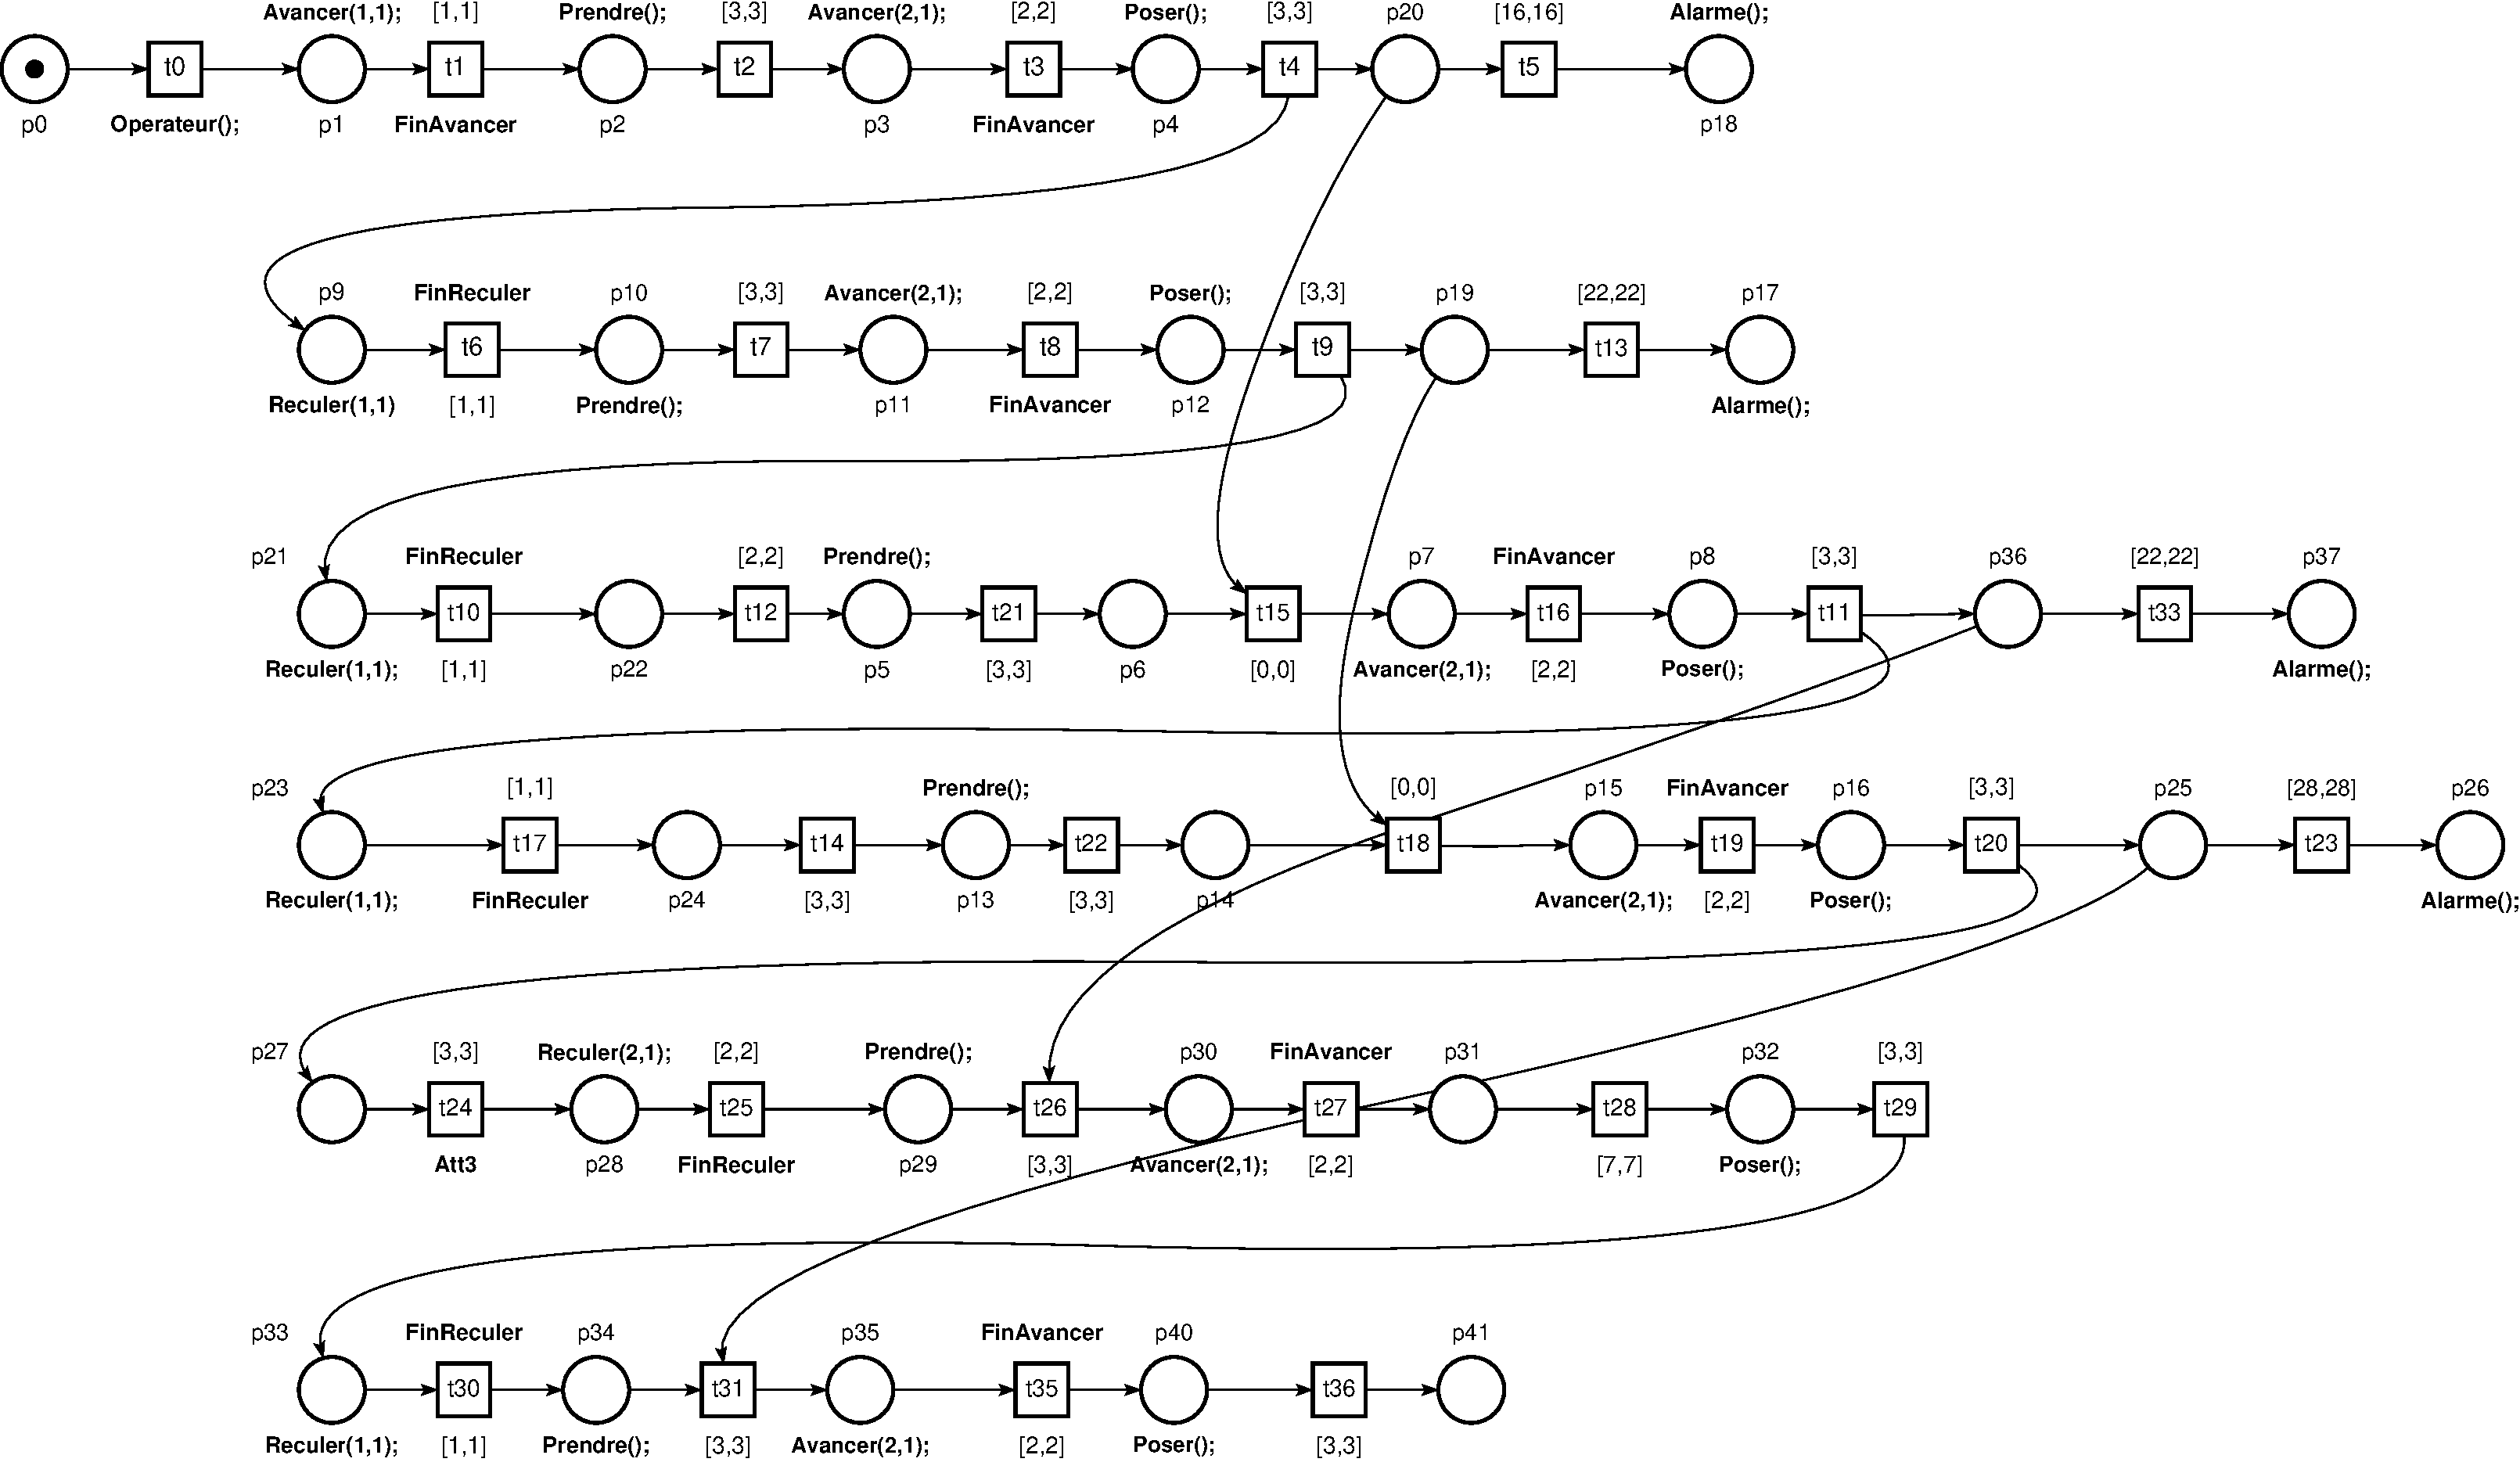
\includegraphics[width=\textwidth]{./III/images/reseau_Analyse--III-3.pdf}
\caption{\label{fig:III-3-rdptCom}Modèle réseau de Petri temporel de commande du STA.}
\end{figure}


Le réseau de Petri Temporel de commande ci-dessus est basé sur le modèle de l'exercice précédent auquel il a été ajouté la séquence pour les 4 autres opérations avec les déclenchement d'alarme nécessaires. Nous avons représenter une ligne par lancement d'opération. Comme expliqué précédemment, nous avons choisi de ne pas considérer les temporisations des opérations $o_5$ et $o_6$, c'est pourquoi les deux dernière ligne du réseau ne contiennent pas de place avec une vérification que la pièce est retirée avant le temps maximal de chaque opération. Les transitions $t_7$, $t_{14}$ et $t_{28}$ contiennent des temporisations afin que le charriot attende de façon à intervenir au bon moment. 
\section{Analyse par graphe de classes}
Afin d'étudier la commande, nous avons ajouté au modèle de commande précédent (figure \ref{fig:III-3-rdptCom}) des temporisations représentants les temps des déplacements (\emph{Avancer()} et \emph{Reculer()}) et les temps de manipulation de pièce (\emph{Prise()} et \emph{Pose()}). Nous obtenons le modèle réseau de Petri temporel suivant (figure \ref{fig:III-3-rdptAnalyse}):
\begin{figure}[!ht]
\centering
\includegraphics[width=\textwidth]{./III/images/reseau_Commande--III-3.pdf}
\caption{\label{fig:III-3-rdptAnalyse}Modèle réseau de Petri temporel de d'analyse de la commande du STA.}
\end{figure}

Nous avons fait une analyse de ce réseau par la méthode du graphe des classes à l'aide de TINA. Cela donne un graphe à 40 classes. Le résultat de l'analyse est disponible en annexe page \pageref{Annex:III}. Nous avons étudier le graphe afin de vérifier que les places activant les alarmes ne sont jamais marquées. Il s'agit des places $p_18$ pour l'opération $o_1$, $p_17$ pour l'opération $o_2$, $p_37$ pour l'opération $o_3$ et $p_26$ pour l'opération $o_4$. Aucune des places déclenchant l'arme n'est marqué n'apparait dans une classe du graphe, donc notre commande ne commet pas d'erreur d'ordonnancement.


\newpage
\section{Implémentation}
Nous n'avons pas eu le temps de réaliser l'implémentation en C de notre modèle de commande. 
Si nous avions eu le temps, nous aurions fait une implémentation de même type que celle proposé en annexe de l'énoncé. Nous aurions créer 3 temporisations pour les transitions $t_7$, $t_{14}$ et $t_{28}$ afin que la commande attende et d'autres pour les transitions $t_{5}$, $t_{13}$, $t_{33}$ et $t_{23}$ nécessaires au déclenchement éventuel de l'alarme.